\documentclass{article}
\usepackage{graphicx} % Required for inserting images
\usepackage{natbib}
\usepackage{hyperref}
\usepackage{array}


\title{Financial Fraud Detection}
\author{Vansh Panchalwar }
\date{April 2026}



\begin{document}

\bibliographystyle{agsm}



\begin{titlepage}
\centering

% Logo (replace filename with your actual logo file)

\includegraphics[width=0.3\textwidth]{images/lbu_logo.png}

\vspace{1cm}

{\Large \textbf{School of Built Environment, Engineering and Computing}}

\vspace{1.5cm}

\renewcommand{\arraystretch}{1.8}

\begin{tabular}{|>{\centering\arraybackslash}m{5cm}|>{\centering\arraybackslash}m{8cm}|}
\hline
\textbf{Student ID} & {c7480107} \\ \hline
\textbf{Student Name} &  {Vansh Panchalwar} \\ \hline
\textbf{Module Name \& CRN} & Machine Learning Techniques for AI - 19889 \\ \hline
\textbf{Level} & 5 \\ \hline
\textbf{Assessment Name} & Coursework \\ \hline
\textbf{Project Title} & Financial Fraud Detection \\ \hline
\textbf{Date of Submission} & 12/05/2025 \\ \hline
\textbf{Course} & BSc Computer Science \\ \hline
\textbf{Academic Year} & 2025--26 S\\ \hline
\end{tabular}

\vfill

{\small 1 | Page}

\end{titlepage}

\section{Introduction}
Financial fraud has become one of the most critical challenge faced by modern finance industry, especially since the rapid growth in online transactions. According to industry reports, global financial fraud losses amount to hundreds of billions of dollars annually, making effective fraud detection systems an essential component of contemporary financial infrastructure.


Traditional fraud detection rely on a set of rules written manually by experts. While these systems are easy to implement, they struggle to adapt to the constantly evolving fraud strategies and often produce high false-positive rates which results in inconvenience and slower transactions. As fraudsters continuously modify their behavior to bypass static rules, machine learning and statistical approaches have increasingly been adopted to detect complex, non-linear patterns in transaction data.

\section{Literature Review}

Financial fraud detection has been widely studied using classic machine learning algorithms such as Logistic Regression, Naïve Bayes, k-Nearest Neighbours (KNN), Decision Trees, and Random Forests. These algorithms are frequently compared due to their complementary characteristics in terms of interpretability, computational complexity, and predictive performance.

Studies also explore different strategies to preprocess data, indicating that preprocessing the data can show massive improvement in performance across various algorithms. 

\subsection{Logistic Regression and Naïve Bayes}

Logistic Regression is one of the earliest and most widely used methods for financial fraud detection due to it's interpretability and performance on binary  classification problems like separating legitimate transactions from fraudulent transactions. Logistic regression is also computationally efficient and has 
good performance on moderately large datasets which makes it a good choice for practical fraud detection \citep{gupta2025fraud}

\subsection{K-Nearest Neighbour (KNN)}

K-Nearest Neighbour (KNN) is an instance based machine learning algorithm in which 

\citet{Itoo2020} evaluated the performance of Logistic Regression against Naïve Bayes and K-Nearest Neighbour (KNN). The results demonstrate Logistic Regression outperforming others with a maximum accuracy of 95\%, while Naïve Bayes and KNN showed a maximum accuracy of 91\% 75\% respectively. The observation also shows that supervised methods such as Logistic Regression and Naïve Bayes have much better fraud detection performance as compared to un-supervised methods like KNN.

These findings are consistent with \citet{arora2023}, who identified Logistic Regression as the better performing method when compared to KNN and Naïve Bayes. 

\subsection{Decision Tree and Random Forest}

Decision Tree is a popular machine learning method because of it's interpretability and performance. For financial fraud detection decision trees can capture complex interaction effects between variables such as transaction amount, account balances, and transaction type. However, studies suggest that their performance can easily degrade due to overfitting, especially on noisy data.

Random Forest is an ensemble learning method based on supervised learning that uses an aggregate of decision trees. Random forest overcomes the shortcomings of decision tree, such as overfitting, by averaging multiple deep decision trees trained on different parts of the same data. 


\citet{khare2018} compared Decision Tree, Random Forest, SVM and Logistic
Regression classifier algorithms based on their accuracy,
sensitivity, specificity and precision. The results indicate that Random Forest outperforms the other methods with an accuracy of 98.6\%, while logistic regression has an accuracy of 97.7\%, SVM shows an accuracy of 97.5\% and the decision tree shows an accuracy of 95.5\%.

The evaluation done by \citet{wang2023} reached the same conclusion, where Random Forest outperforms Logistic Regression with an outstanding  precision of 100\%, which is near perfect while Logistic Regression had a precision of 90\%. \citet{wang2023} also highlighted the importance of locating well labeled data, as required by supervised learning methods like Logistic Regression and Random Forest. In absence of labeled data, \cite{wang2023} recommends considering unsupervised learning as an alternative. 

\citet{popova2025creditcardfrauddetection} also highlighted the importance of preprocessing the data, demonstrating that using undersampling, SMOTE, and a hybrid approach, evaluated by \citet{Hybrid}, to preprocess data to train the model can improve the performance upto 23\% some cases.

This aligns with the study done by \citet{idrees2024credit}, who also explored alternative data preprocessing strategies to improve model performance. 

\section{Exploratory Data Analysis}

\subsection{Data Overview}

The dataset consists of 24,192 financial transactions described by 11 variables. These 11 variables include transaction attributes, balance before and after transaction, and a binary fraud indicator (\texttt{isFraud}). This dataset has both numerical and categorical variables 

\subsection{Data structure and Quality}

Inspection using \texttt{str()} reveals that the dataset contains a mixture of numerical variables such as \texttt{amount}, balance before and after transaction stored and categorical values like \texttt{type}. 

\subsection{Missing Values}
Missing values were observed in several variables. Numerical variables such as \texttt{amount} and balance, before and after transaction, all show missing values as indicated by the number of observations in \texttt{str()} output. Categorical variables such as \texttt{Amount.Category} and \texttt{type} contain missing values, indicated by the presence of empty strings in the dataset.

Empty strings in \texttt{Amount.Category} and \texttt{type} were converted into NA to enable consistent visualization of missingness across the variables. A missingness heatmap was then generated using \texttt{missmap()} function provided by the \texttt{Amelia} package to visualize missingness across the dataset.

Figure~\ref{fig:missmap} illustrates the pattern of missing data across variables.

\begin{figure}[htbp]
    \centering
    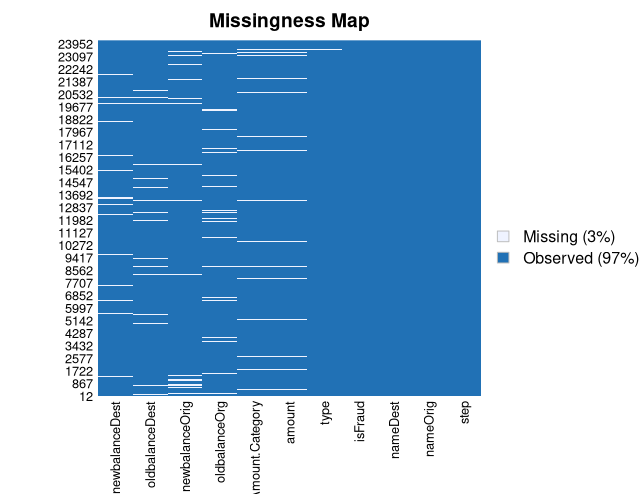
\includegraphics[width=0.7\linewidth]{images/missmap2.png}
    \caption{Missing value heatmap of the dataset}
    \label{fig:missmap}
\end{figure}

The figure shows that most of the dataset is complete, with missing values only covering 3\% of the dataset. The missing values however, are not random across the variables as indicated by the horizontal patterns in the figure. These patterns are commonly observed in synthetically modified data, suggesting that our dataset might be preprocessed.

Missingness is primarily concentrated in balance related variables and transaction type, while variables like the account names, \texttt{step} and \texttt{isFraud} are fully obeserved.


\subsection{Bivariate Analysis}

Bivariate Analysis was conducted to observe the relationship between selected variables and target variable \texttt{isFraud}. The variables were chosen based on their relevance to fraud detection.

\subsubsection{Transaction Type and Fraud}

Transaction type was selected due to it's categorical nature and it's association with fraudulent activities. Different transaction types are expected to carry a different risk of fraud.

Figure~\ref{fig:fraud_type} visualizes the proportion of fraud and non fraud transactions in the dataset.

\begin{figure}[htbp]
    \centering
    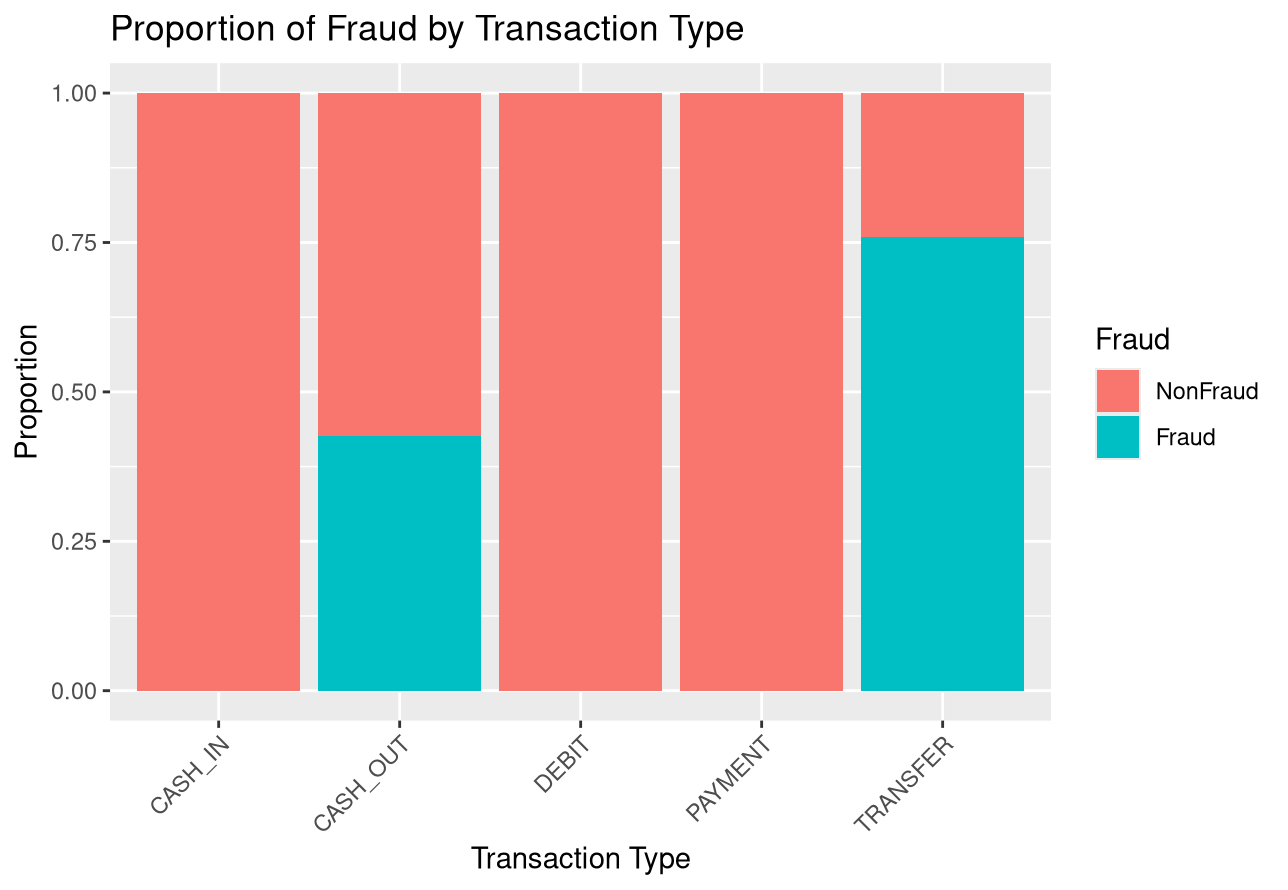
\includegraphics[width=0.7\linewidth]{images/fraud01_type_no_miss.png}
    \caption{Proportion of fraud by Transaction Type}
    \label{fig:fraud_type}
\end{figure}

From the figure we can observe that fraudulent transactions are mostly concentrated in \texttt{Transfer} and \texttt{Cash\_Out} transaction types. This indicated that transaction type can be a strong indicator of fraudulent behavior and should be retained as an important variable in model training.

\subsubsection{Transaction Amount and Fraud}

Figure~\ref{fig:amount_fraud} illustrates the distribution of transaction amounts by fraud status using a logarithmic scale.

\begin{figure}[htbp]
    \centering
    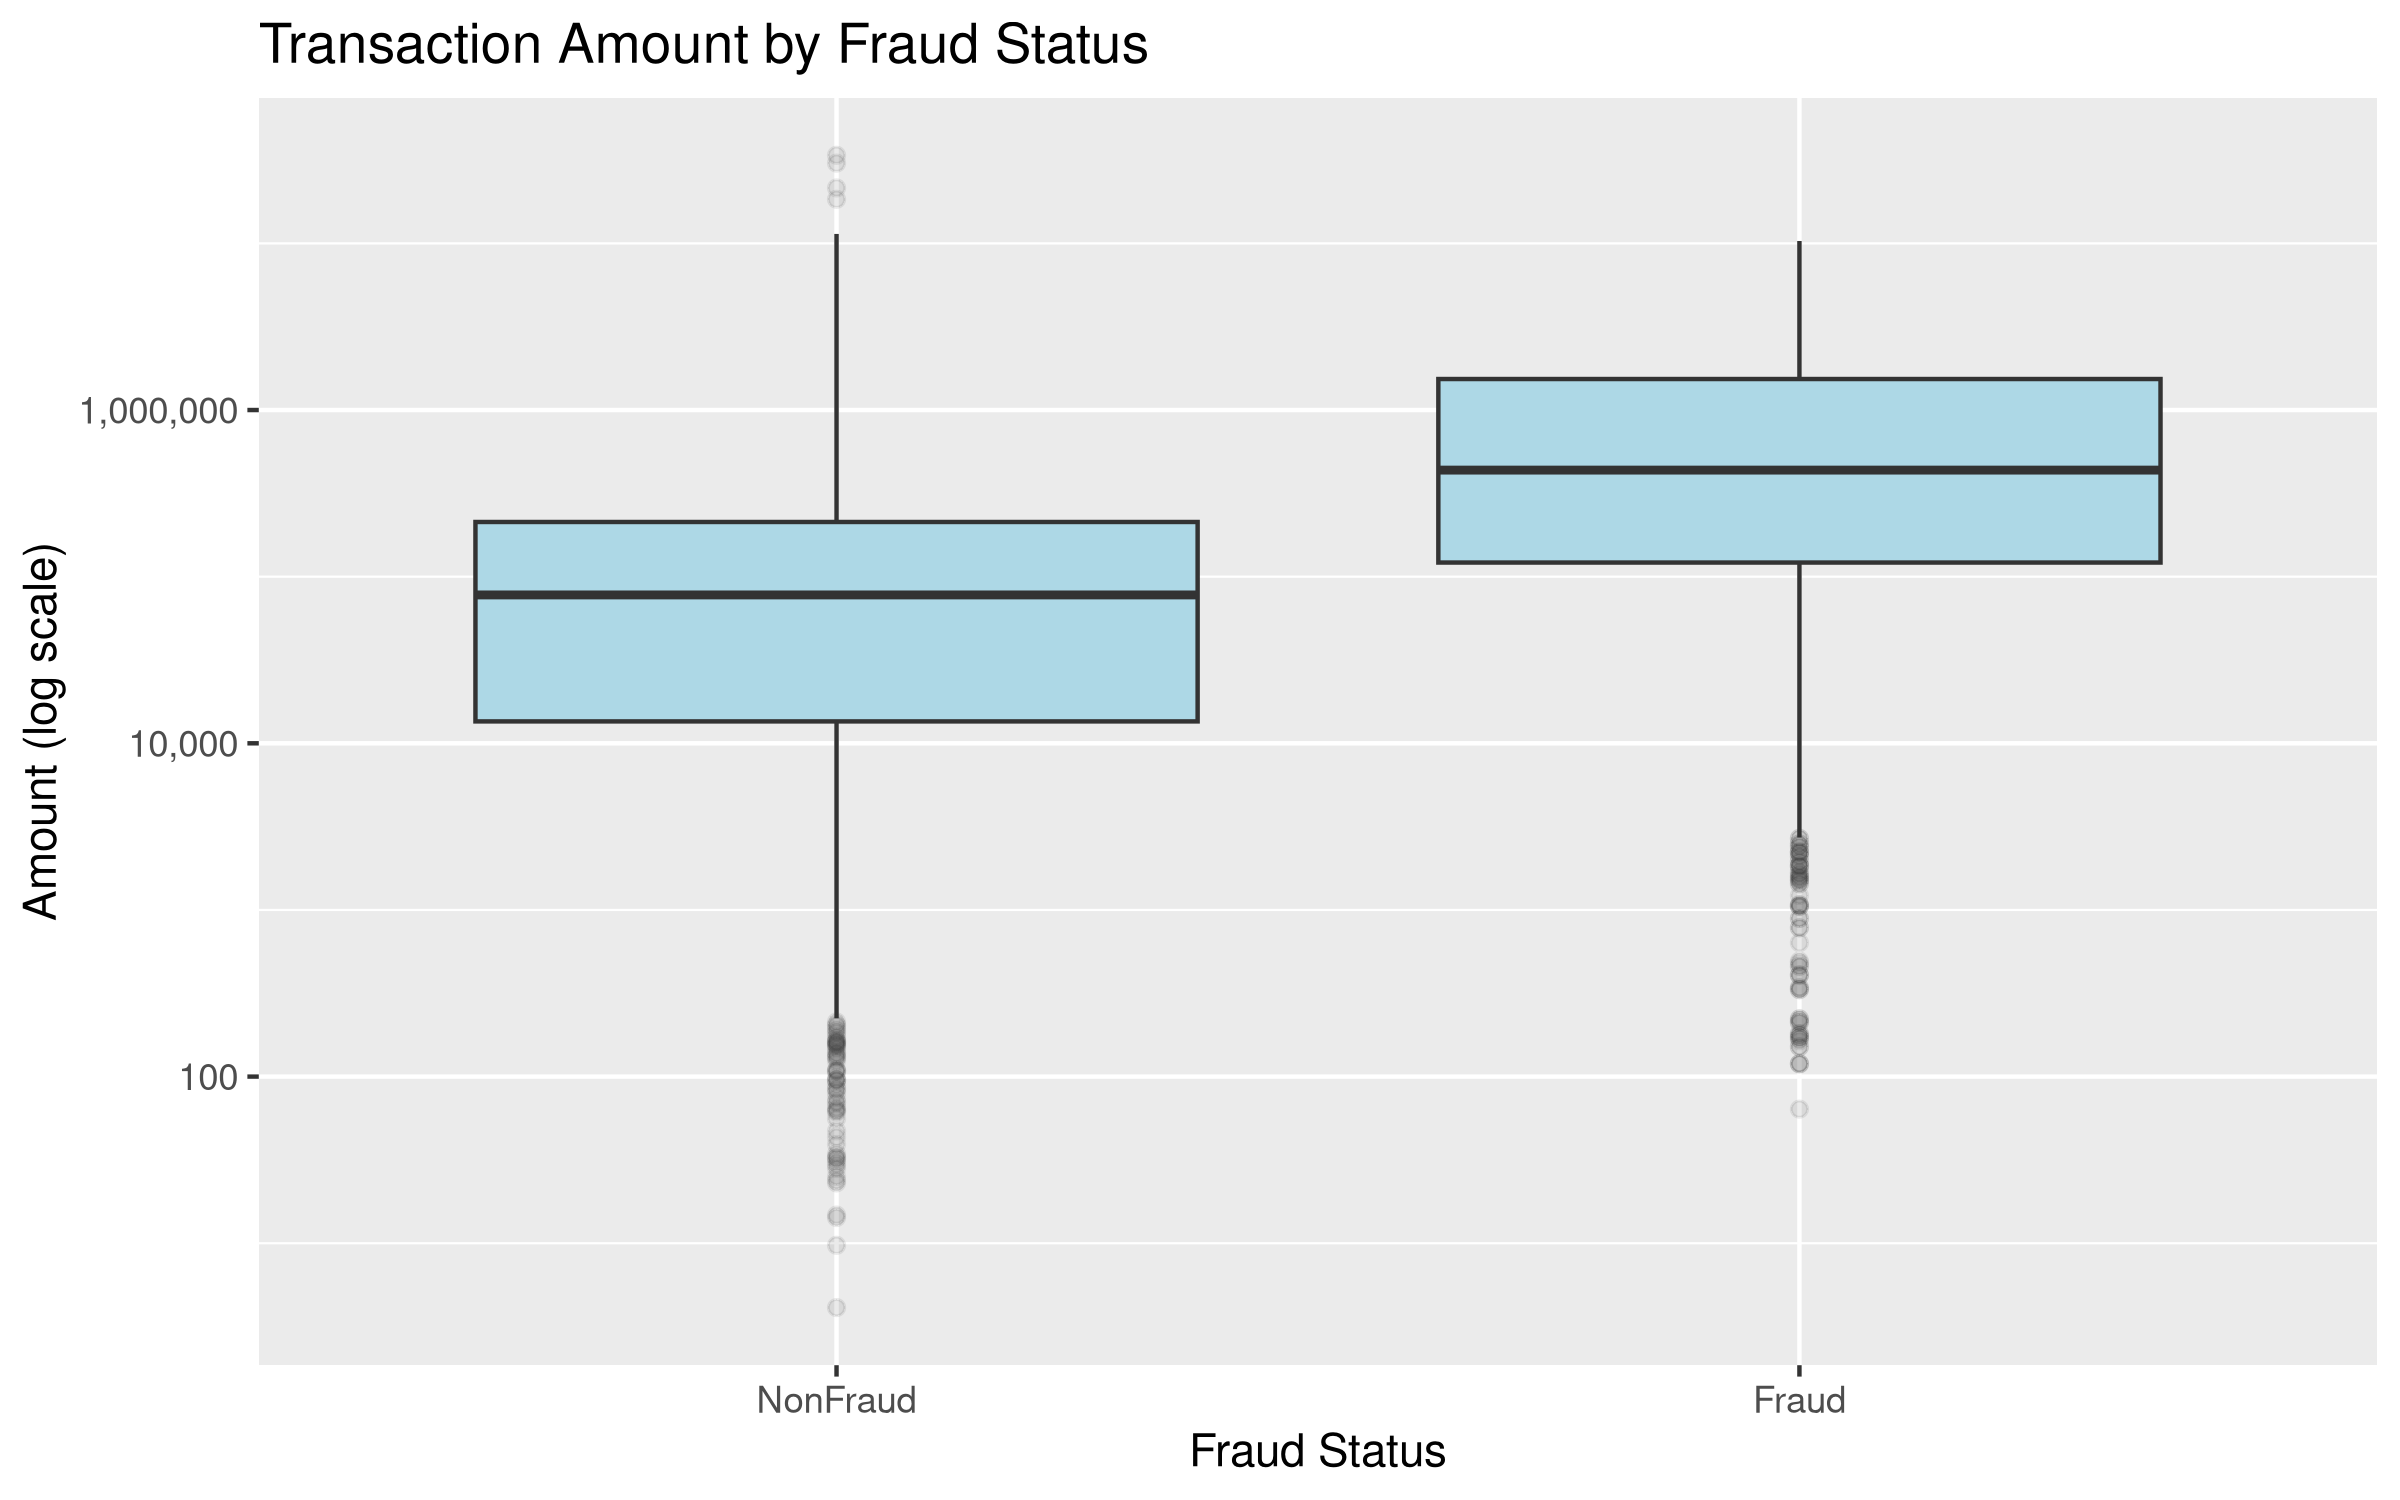
\includegraphics[width=0.7\linewidth]{images/amount_fraud.png}
    \caption{Transaction Amount by Fraud Status}
    \label{fig:amount_fraud}
\end{figure}

The figure visualizes the relationship between transaction amount and fraud. The presence of outliers is visualized, with extreme high and low values in both cases. We can observe that fraudulent transactions are generally associated with higher transaction amounts compared to non-fraudulent transactions, as indicated by the median transaction value of fraud cases. 

\subsubsection{Amount Category and Fraud}

The transactions in the dataset are categorized into low, medium and high by \texttt{Amount.Category}. Figure~\ref{fig:amount_category} visualizes this relationship.

\begin{figure}[htbp]
    \centering
    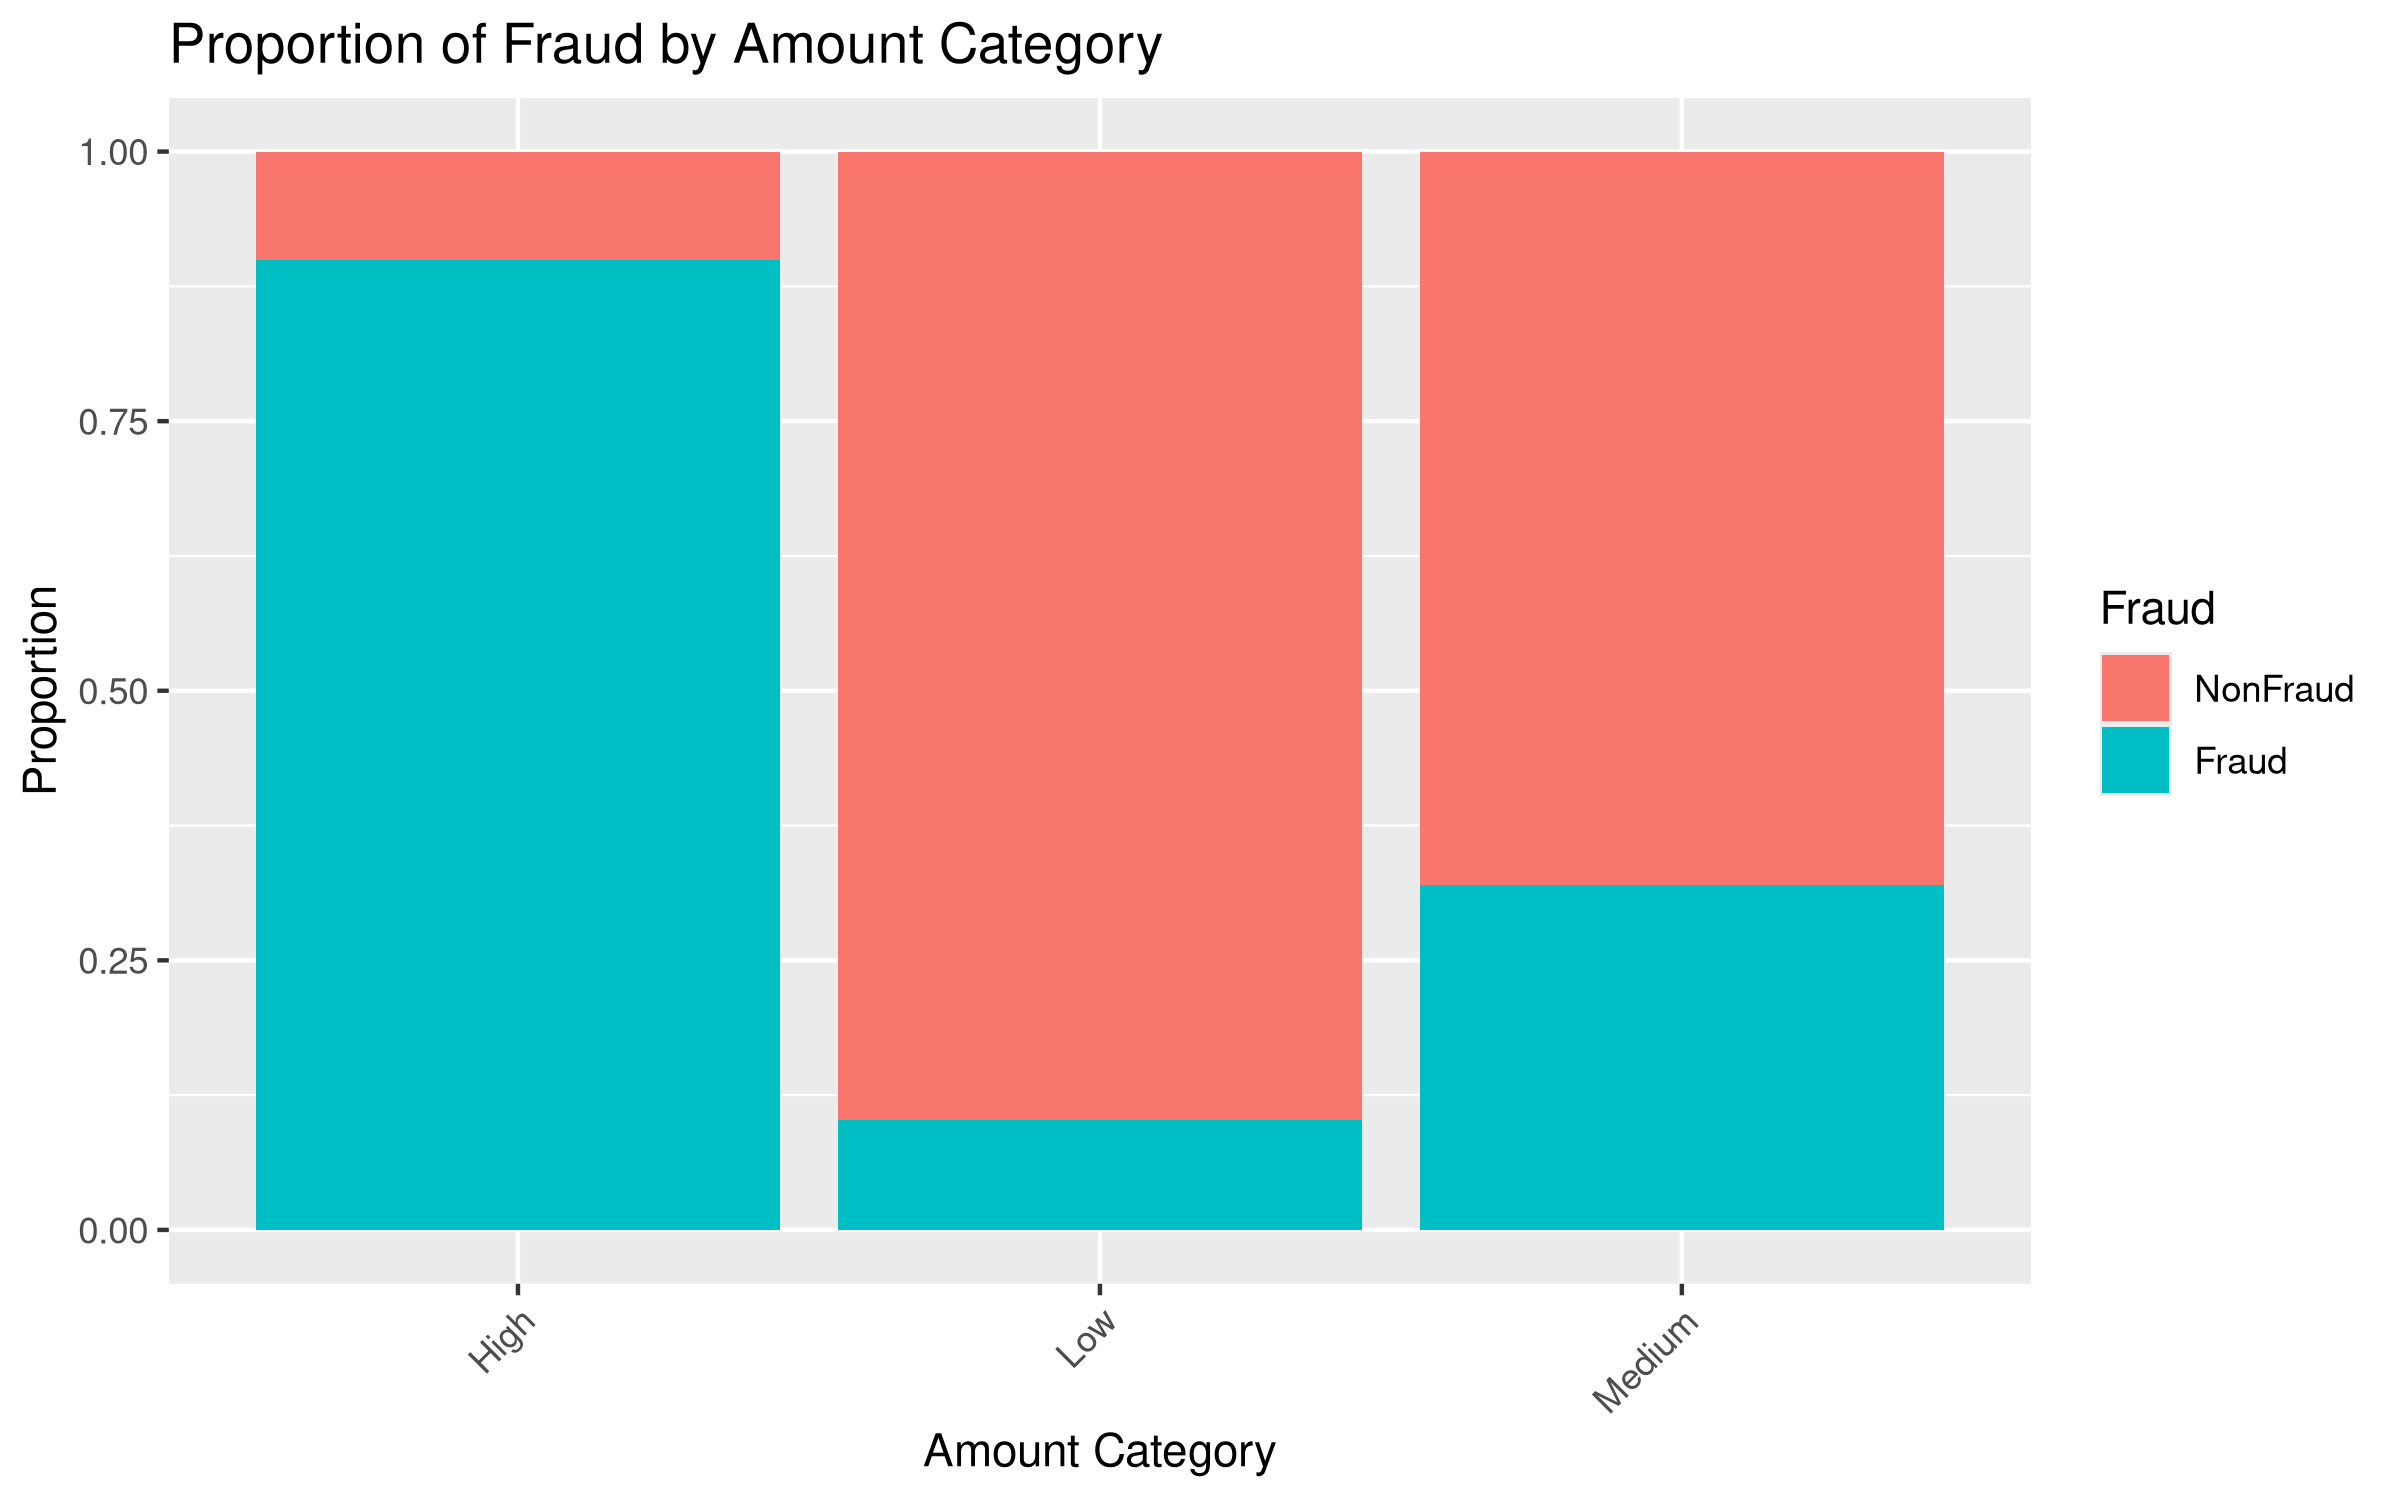
\includegraphics[width=0.7\linewidth]{images/amount_category.png}
    \caption{Proportion of fraud by Amount Category}
    \label{fig:amount_category}
\end{figure}

From the figure we can observe that fraud transactions are mostly concentrated in the high amount category. This aligns with our previous findings indicating fraudulent transactions are usually associated with medium to high amounts, while the low amount category sees lower fraudulent bevaiour comparatively. 


\subsection{Summary of EDA Findings}

The exploratory data analysis highlights several important characteristics of the dataset. Missing values are present but limited to a relatively small proportion, and are concentrated in specific variables rather than randomly distributed. Transaction amounts and balance-related variables exhibit strong skewness and contain extreme values.

Bivariate analysis reveals that fraudulent transactions are not uniformly distributed across the dataset. Instead, they are concentrated in specific transaction types such as \texttt{TRANSFER} and \texttt{CASH\_OUT}, and are generally associated with higher transaction amounts.

These findings indicate that variables such as transaction type, transaction amount, and balance-related features are likely to be important predictors of fraud, and therefore should be retained for further modelling.

\section{Data Pre-processing and Feature Engineering}

\subsection{Outlier Detection}

Outliers were observed using the Interquartile Range (IQR) method applied to the \texttt{amount} variable. 2616 outliers were observed representing transactions that fall significantly outside the typical range. Figure~\ref{fig:amount_fraud} visualizes the extreme values in both cases.

Due to the highly skewed nature of transaction amounts, a standard boxplot produced a compressed visualisation dominated by extreme values. To improve interpretability, a logarithmic transformation was applied to the transaction amounts when visualising the data. 

These outliers were retained in the dataset. In the context of fraud detection, unusually large or small transaction amounts often represent anomalous or fraudulent behaviour, and removing them may reduce the model's ability to detect such patterns.

\subsection{Multicollinearity}

To assess relationships between numerical predictor variables, a correlation matrix was computed and visualised using a heatmap. 

\begin{figure}[htbp]
    \centering
    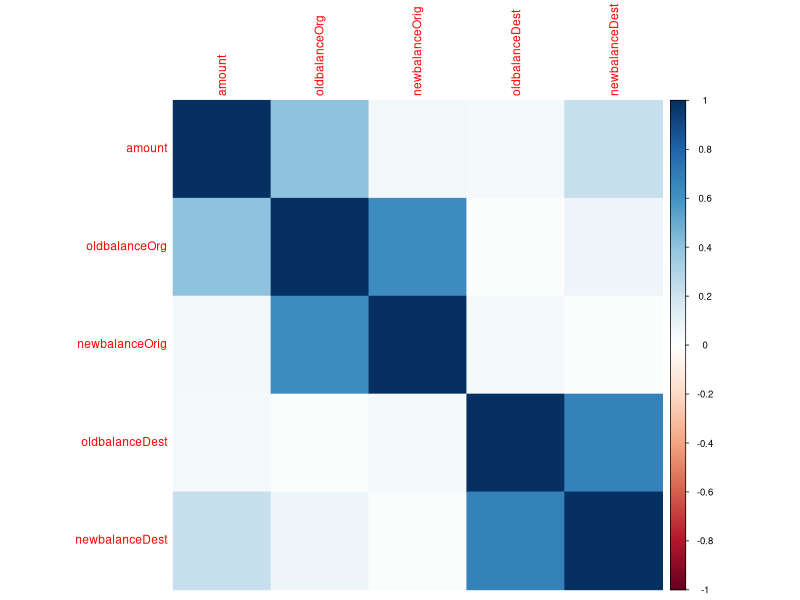
\includegraphics[width=0.5\linewidth]{images/correlation_plot.png}
    \caption{Correlation between variables}
    \label{fig:correlation}
\end{figure}

The analysis reveals strong correlations between balance related variables between \texttt{oldbalanceOrg} and \texttt{newbalanceOrig}, and between \texttt{oldbalanceDest} and \texttt{newbalanceDest}. This is expected, as post-transaction balances are directly influenced by pre-transaction balances and transaction amounts.

Although these correlations suggest potential redundancy, the variables were retained because they capture important transactional behaviour that may improve model performance.


\subsection{Variable Selection}

Some variables were identified as unsuitable for modelling. In particular, \texttt{nameOrig} and \texttt{nameDest} were removed from the dataset. These variables represent anonymised account identifiers with high cardinality, meaning they contain a large number of unique values.

Such variables do not provide meaningful predictive information and may introduce noise or lead to overfitting. After removing these variables, a reduced dataset (\texttt{FT\_model}) was obtained, containing only relevant features for modelling.

\subsection{Encoding and Scaling}

Categorical variables like \texttt{type}, \texttt{Amount.Category}, and \texttt{isFraud}, were converted into factor variables to ensure proper handling by classification algorithms.

Numerical variables were standardised using feature scaling. Scaling ensures that all variables contribute equally to model training, which is particularly important for algorithms such as K-Nearest Neighbours and Logistic Regression since they are sensitive to the magnitude of input features.

Tree-based models such as Decision Trees and Random Forest are not affected by scaling, however, a consistent preprocessing approach was applied across all models for simplicity and comparability.

The resulting dataset (\texttt{FT\_model}) is therefore clean, consistent, and suitable for further modelling.

\section{Modelling}

\subsection{Model Development}

Five classification models were developed to predict fraudulent transactions: Logistic Regression, K-Nearest Neighbours (KNN), Naïve Bayes, Decision Tree, and Random Forest. 

The dataset was split into training and testing sets using a 70/30 partition. This ensures that model performance can be evaluated on unseen data, providing a realistic assessment of predictive capability.

To improve model reliability and reduce overfitting, we use a 5-fold cross-validation during the training. The dataset was divided into five equal subsets, where each subset was used once as validation data while the remaining subsets were used for training. The choice of 5-fold cross-validation provides a good balance between computational efficiency and robustness of results.

Hyperparameter tuning was incorporated using the \texttt{tuneLength} parameter in the modelling process. This allows the models, particularly KNN, Decision Tree, and Random Forest, to explore different parameter values and automatically select the best performing configuration.

The primary evaluation metric used was the Area Under the ROC Curve (AUC). AUC is particularly suitable for fraud detection as it evaluates the ability of the model to distinguish between classes across all classification thresholds, which is important in imbalanced datasets where accuracy alone may be misleading. Additional metrics such as sensitivity and specificity were also considered to assess model performance.

\subsection{Cross-Validation Results}

The performance of each model under cross-validation is summarised below.

The results indicate that Random Forest achieved the best overall performance, with a mean ROC value of approximately 0.9989. KNN and Decision Tree also performed strongly, achieving ROC values of approximately 0.9736 and 0.9728 respectively. Logistic Regression achieved moderate performance with a mean ROC of approximately 0.9248, while Naïve Bayes had the lowest performance at approximately 0.9090. Table ~\ref{tab:roc_cv} visualizes the results

\begin{table}[htbp]
\centering
\begin{tabular}{lcccccc}
\hline
Model & Min & Q1 & Median & Mean & Q3 & Max \\
\hline
Logistic Regression & 0.9193 & 0.9213 & 0.9248 & 0.9248 & 0.9260 & 0.9326 \\
KNN                 & 0.9723 & 0.9724 & 0.9734 & 0.9736 & 0.9743 & 0.9758 \\
Naïve Bayes         & 0.9032 & 0.9046 & 0.9066 & 0.9090 & 0.9127 & 0.9181 \\
Decision Tree       & 0.9675 & 0.9703 & 0.9709 & 0.9728 & 0.9767 & 0.9787 \\
Random Forest       & 0.9981 & 0.9986 & 0.9990 & 0.9989 & 0.9994 & 0.9994 \\
\hline
\end{tabular}
\caption{Cross-validation ROC results for all models}
\label{tab:roc_cv}
\end{table}

This aligns with the results in the studies done by \citet{khare2018}, but differs with the study done by \citet{Itoo2020}. In the evaluation done by \citet{Itoo2020}, Logistic regresssion and Naive Bayes performed better than KNN.


Analysis of sensitivity and specificity provides further insight into model behaviour. Naïve Bayes achieved very high sensitivity (approximately 0.9946), meaning it is highly effective at identifying fraudulent transactions. However, it exhibits very low specificity (approximately 0.2280), indicating a high rate of false positives. This makes it unsuitable for practical use in fraud detection, where incorrectly flagging legitimate transactions can be costly. Table ~\ref{tab:sens_cv} summarises the sensitivity performance of all models 

\begin{table}[htbp]
\centering
\begin{tabular}{lcccccc}
\hline
Model & Min & Q1 & Median & Mean & Q3 & Max \\
\hline
Logistic Regression & 0.9010 & 0.9091 & 0.9104 & 0.9105 & 0.9150 & 0.9168 \\
KNN                 & 0.9598 & 0.9651 & 0.9662 & 0.9653 & 0.9674 & 0.9680 \\
Naïve Bayes         & 0.9930 & 0.9936 & 0.9948 & 0.9946 & 0.9953 & 0.9965 \\
Decision Tree       & 0.9639 & 0.9686 & 0.9721 & 0.9724 & 0.9779 & 0.9796 \\
Random Forest       & 0.9866 & 0.9884 & 0.9884 & 0.9891 & 0.9901 & 0.9919 \\
\hline
\end{tabular}
\caption{Cross-validation sensitivity results}
\label{tab:sens_cv}
\end{table}


In contrast, Random Forest achieved both high sensitivity (approximately 0.9891) and high specificity (approximately 0.9901), demonstrating balanced performance across both classes. Decision Tree and KNN models also showed strong and balanced performance, though slightly lower than Random Forest.

Logistic Regression demonstrated reasonable performance but was limited by its assumption of linear relationships between predictors and the target variable, which may not capture the complexity of fraud patterns.

\subsection{Test Set Evaluation}

To evaluate how well the models generalise to unseen data, performance was assessed on the test dataset. The AUC values for all models are presented in Table~\ref{tab:auc}.

\begin{table}[htbp]
\centering
\begin{tabular}{lc}
\hline
Model & AUC \\
\hline
Logistic Regression & 0.9183 \\
KNN & 0.9749 \\
Naïve Bayes & 0.9067 \\
Decision Tree & 0.9667 \\
Random Forest & 0.9986 \\
\hline
\end{tabular}
\caption{Model performance on the test dataset}
\label{tab:auc}
\end{table}

The test results confirm the patterns observed in cross-validation. Random Forest achieves the highest AUC (0.9986), indicating near-perfect classification performance. KNN and Decision Tree also perform strongly, with AUC values exceeding 0.96.

Logistic Regression again shows moderate performance, while Naïve Bayes performs the weakest. The consistency between cross-validation and test results suggests that the models are not overfitting and are generalising well to new data.

Overall, most of our results align with the findings in the literature review.

\subsection{ROC Curve Analysis}

Figure~\ref{fig:roc} presents the ROC curves for all models.

\begin{figure}[htbp]
\centering
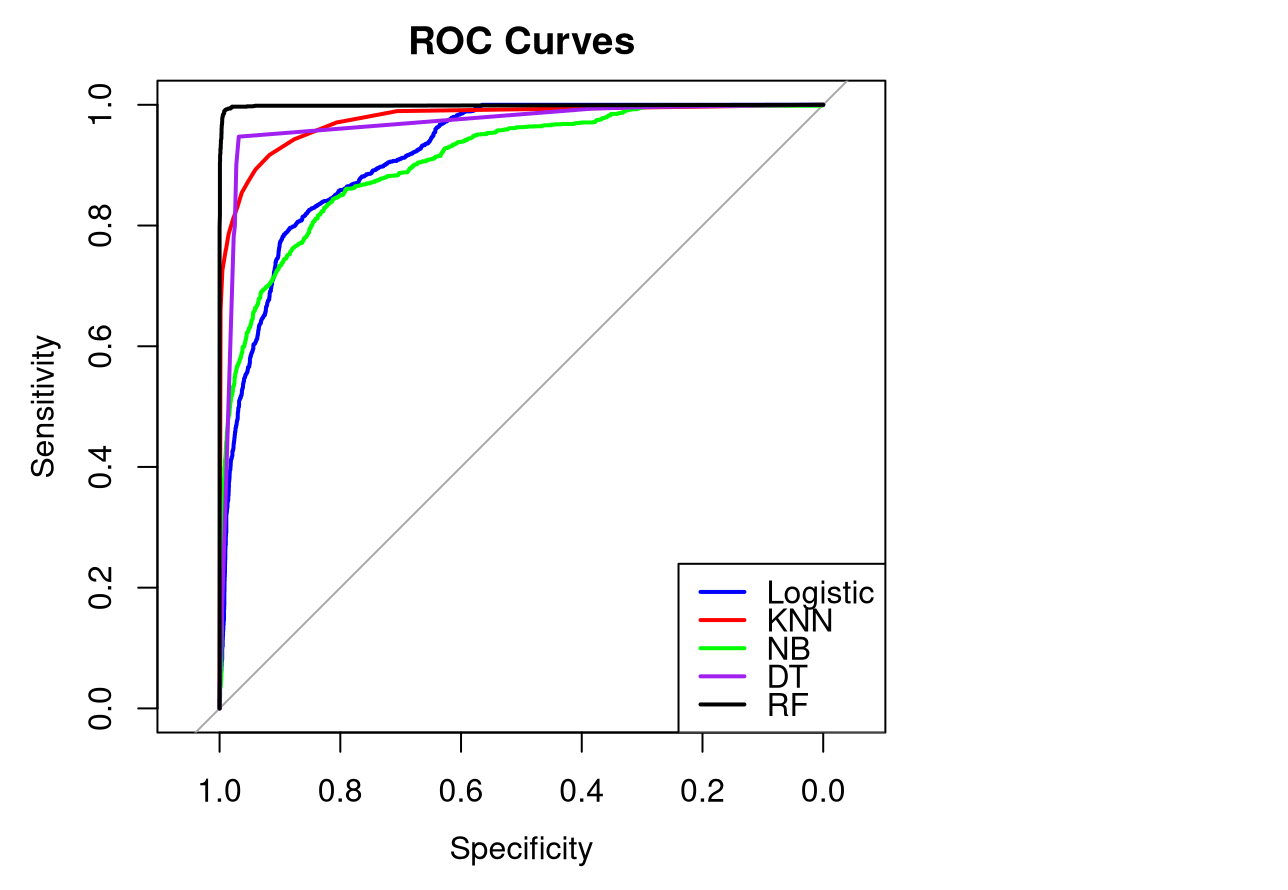
\includegraphics[width=0.7\linewidth]{images/ROC1.png}
\caption{ROC curves for all models}
\label{fig:roc}
\end{figure}

The ROC curves illustrate the trade-off between sensitivity and specificity across different models. The Random Forest model is closest to the top-left corner, indicating superior performance with both high true positive and low false positive rates.

Decision Tree and KNN also exhibit strong performance, with curves close to the optimal region. Logistic Regression shows lower performance, while Naïve Bayes performs worst among the models. These results reinforce the findings from the AUC analysis.

\subsection{Model Comparison}

Overall, the Random Forest model consistently outperforms all other models across multiple evaluation metrics, including AUC, sensitivity, and specificity. As shown in Table~\ref{tab:auc} and Figure~\ref{fig:roc}, Random Forest achieves the highest predictive performance, with near-perfect classification capability. This can be attributed to its ensemble nature, where multiple decision trees are combined to improve accuracy and reduce overfitting.

K-Nearest Neighbours and Decision Tree models also perform well, with relatively high AUC values, suggesting that non-linear relationships play a significant role in fraud detection. These models are able to capture complex patterns in the data more effectively than linear approaches.

Logistic Regression, being a linear model, demonstrates moderate performance. This indicates its limitation in capturing the non-linear relationships present in the dataset, which are important for distinguishing fraudulent transactions.

Naïve Bayes, despite achieving high sensitivity, suffers from poor specificity. This indicates that it produces a high number of false positives. The weakness of Naïve Bayes can be attributed to its assumption of feature independence, which does not hold strongly in this dataset, particularly given the presence of correlated balance variables.

These results suggest that models capable of capturing complex and non-linear patterns, particularly ensemble methods such as Random Forest, are better suited for fraud detection tasks.

\section{Conclusion}

This study evaluated the performance of several machine learning models for detecting fraudulent financial transactions, including Logistic Regression, K-Nearest Neighbours (KNN), Naïve Bayes, Decision Tree, and Random Forest. The results demonstrate that more advanced models, particularly ensemble methods, significantly outperform simpler approaches.

In comparison with the models discussed in the literature review, the findings are consistent. Logistic Regression showed moderate performance due to its linear nature, while Naïve Bayes exhibited high sensitivity but poor specificity, reflecting its strong independence assumptions. In contrast, KNN and Decision Tree models performed well, confirming that non-linear approaches are more suitable for fraud detection. The Random Forest model achieved the best performance overall, with the highest AUC and a strong balance between sensitivity and specificity.

The exploratory and preprocessing stages highlighted the importance of several key variables. Transaction type, transaction amount, and balance-related variables were identified as strong indicators of fraudulent behaviour. In particular, transaction type provided clear separation between classes, with fraud concentrated in specific categories such as \texttt{TRANSFER} and \texttt{CASH\_OUT}. Transaction amount also showed good discriminatory power, with fraudulent transactions generally occurring at higher values. Although balance variables exhibited high correlations, they were retained as they represent meaningful financial relationships rather than redundant information.

These findings align with previously published work, which suggests that ensemble methods and non-linear models are more effective for fraud detection tasks. The strong performance of Random Forest in this study further supports this conclusion.

Future research could explore more advanced techniques, such as better data preprocessing, to further improve predictive performance. Additionally, incorporating more complex feature engineering, such as temporal patterns or user behaviour analysis, may enhance model accuracy. Improving methods for handling class imbalance could also further strengthen fraud detection performance.

Overall, this study demonstrates that machine learning models, particularly Random Forest, are highly effective when applied to well-preprocessed financial transaction data.


\bibliography{references/LR_citation-392331388,references/NB_citation-339294125,references/Khare,references/NB___citation-374121256,references/LR_vs_RF_citation-374638842,references/popova,references/Hybrid,references/IJCS}


\clearpage
\section*{Appendix A}

\begin{center}
    {\Large \textbf{Appendix A}}\\[0.5cm]
    {\large \textbf{Originality and Use of Generative Artificial Intelligence (GAI) Statement}}
\end{center}

\vspace{0.5cm}

\begin{itemize}
    \item I understand that to use the work and ideas of others, including generative AI output, without full acknowledgement, is academic unfair practice.

    \item I confirm that this coursework submission is all my own, original work and that all sources, summaries, paraphrases and quotes are fully referenced as required by the LBU Academic Regulations.
\end{itemize}

\vspace{0.5cm}

\textbf{DECLARATION OF GENERATIVE AI USE (This is an example, you can modify, adapt, delete as appropriate):}

\vspace{0.3cm}

I did use Generative AI technology in the development, writing, or editing of this assignment. I have included a copy of the reference used, and the output generated in the Appendix section. If you have any concerns about whether you have used generative AI tools (in)correctly, please seek advice before submitting your assignment from academic staff responsible for the assessment that this submission relates to. The shaded boxes are examples to help you with completing this section.

\vspace{0.8cm}

\renewcommand{\arraystretch}{1.5}

\begin{tabular}{|p{2cm}|p{3cm}|p{4cm}|p{4cm}|}
\hline
\textbf{Numbering} & \textbf{Generative AI Tool (e.g. ChatGPT)} & \textbf{How generative AI Tool was used} & \textbf{Reference} \\ 
\hline

1 & Microsoft Copilot 365 & 
Asked for assistance with literature formatting and code formatting & 
\url{https://copilot.microsoft.com/} \\ 
\hline

2 & Microsoft Copilot 365 & 
Assistance with LaTeX syntax and formatting. & 
\url{https://copilot.microsoft.com/} \\ 
\hline

\end{tabular}

\end{document}
